%%%%%%%%%%%%%%%%%%%%%%%%%%%%%%%
\section{Numerical scan of the parameter space}

\subsection{Results for the generic scan}
To have a complete picture of the properties of i2HDM in the whole parameter space, we have performed a
five-dimensional random scan of the model parameter space with about $10^8$ points, evaluating all relevant
observables and limits mentioned above. The range for 
the model parameters of the scan was chosen according to the Eq.~(\ref{eq:scan-limits}).

%\begin{table}[ht]
%\begin{center}
%\begin{tabular}{|c|c|c|}
%\hline
%Parameter      & min value &  max value \\ \hline 
%Mh$_1$ [GeV]   &    10	&     1000  \\ \hline
%Mh$_2$ [GeV]   &    10	&     1000  \\ \hline
%Mhc [GeV]      &    10	&    1000  \\ \hline
%$\lambda_{345}$&  $-8\pi$  &    $8\pi$  \\ \hline
%$\lambda_2$    &   $-8\pi$ &     $8\pi$   \\ \hline
%\end{tabular} 
%\end{center}
%\caption{Range for the wide scan of the parameter space. \label{tab:wide-scan}}
%\end{table}


To better delineate the impact of each constraint, we have imposed different cuts on the parameter space sequentially, 
following the classification below:
\begin{itemize}
\item[Cut-1:] theoretical constraints on the potential from vacuum stability 
[Eq.(\ref{eq:scalar-pot1}-\ref{eq:scalar-pot2}) and (\ref{eq:l345-vacuum-stab})], perturbativity  and
unitarity [Eq.(\ref{eq:unit}-\ref{eq:l345max})];
\item[Cut-2:] constraints from LEP [Eq.~(\ref{eq:constr-widths}) and (\ref{eq:dmh12})], EWPT
[Eq.~(\ref{eq:ewpt})] and the LHC Higgs data
[Eq.~(\ref{eq:lhc-higgs-invis}-\ref{eq:lhc-higgs-aa})];
\item[Cut-3:] constraint on the relic
density  [$\Omega_{\rm DM} h^2 \le 0.1184+2\times 0.0012$], where we consider only the upper bound within 2 standard deviations;
\item[Cut-4:] constraints from DM DD searches from LUX.
\end{itemize}


\begin{figure}[htb]
\vskip -1.0cm
\hspace*{-0.3cm}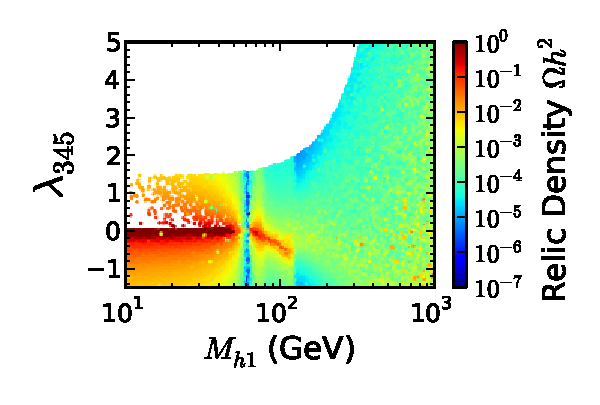
\includegraphics[width=0.41\textwidth]{Figures/Mh1_ld345_Omega_large-cut12.pdf}%
\hspace*{-1.78cm}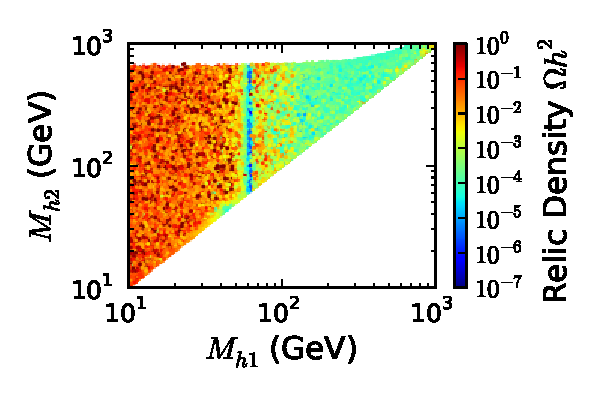
\includegraphics[width=0.41\textwidth]{Figures/Mh1_Mh2_Omega_large-cut12.pdf}%
\hspace*{-1.77cm}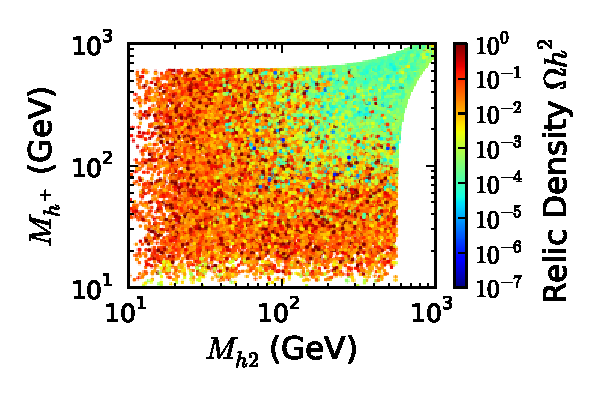
\includegraphics[width=0.41\textwidth]{Figures/Mhc_Mh2_Omega_large-cut12.pdf}%
\vskip -1.1cm
\hspace*{1.2cm}(a)\hspace*{0.35\textwidth}\hspace*{-1.3cm}(b)\hspace*{0.35\textwidth}\hspace*{-1.2cm}(c)
\vskip 0.0cm
{\hspace*{-0.3cm}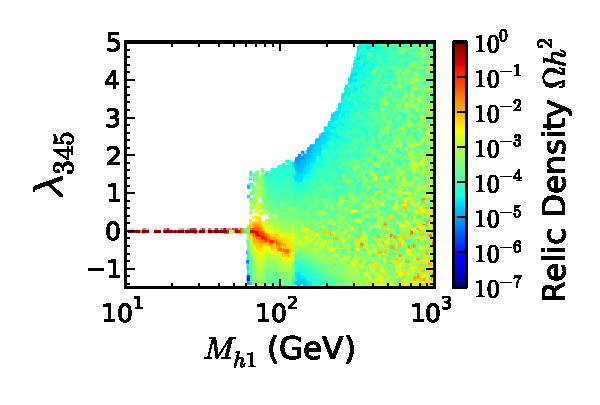
\includegraphics[width=0.41\textwidth]{Figures/Mh1_ld345_Omega_large-cut123456.pdf}}%
{\hspace*{-1.78cm}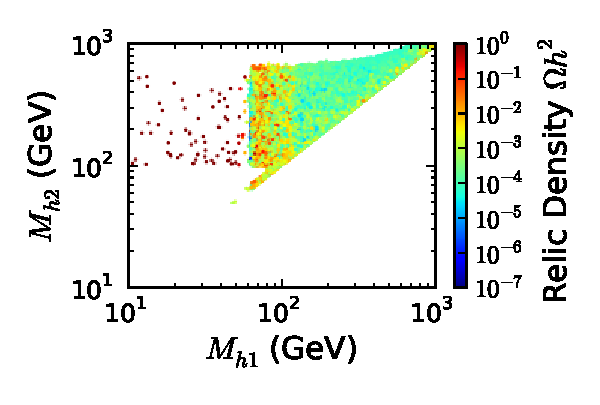
\includegraphics[width=0.41\textwidth]{Figures/Mh1_Mh2_Omega_large-cut123456.pdf}}%
{\hspace*{-1.77cm}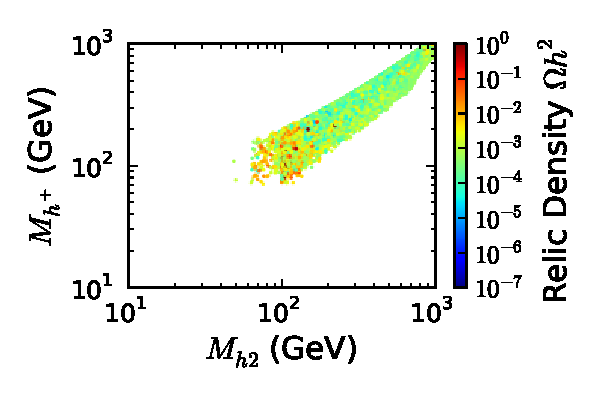
\includegraphics[width=0.41\textwidth]{Figures/Mhc_Mh2_Omega_large-cut123456.pdf}}%
\vskip -1.1cm
\hspace*{1.2cm}(d)\hspace*{0.35\textwidth}\hspace*{-1.3cm}(e)\hspace*{0.35\textwidth}\hspace*{-1.2cm}(f)
\vskip 0.0cm
{\hspace*{-0.3cm}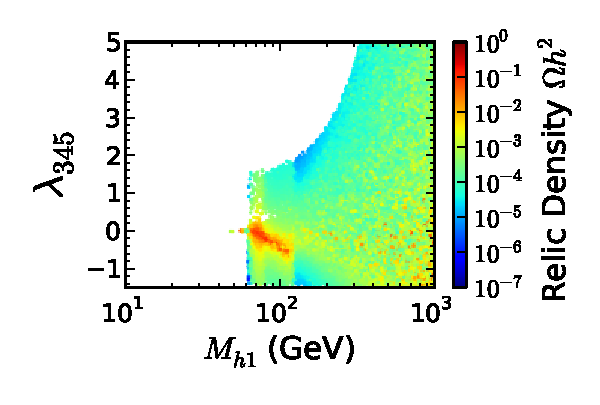
\includegraphics[width=0.41\textwidth]{Figures/Mh1_ld345_Omega_large-cut1234567.pdf}}%
{\hspace*{-1.78cm}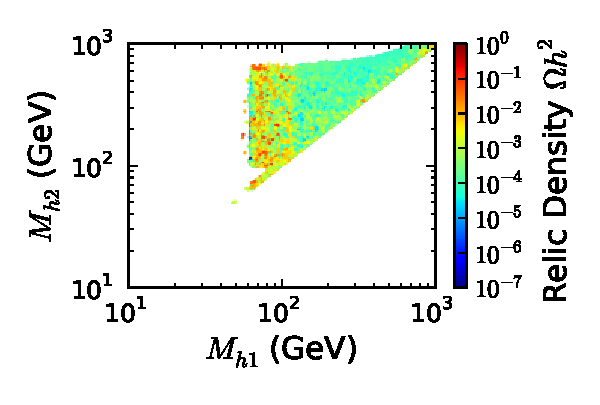
\includegraphics[width=0.41\textwidth]{Figures/Mh1_Mh2_Omega_large-cut1234567.pdf}}%
{\hspace*{-1.77cm}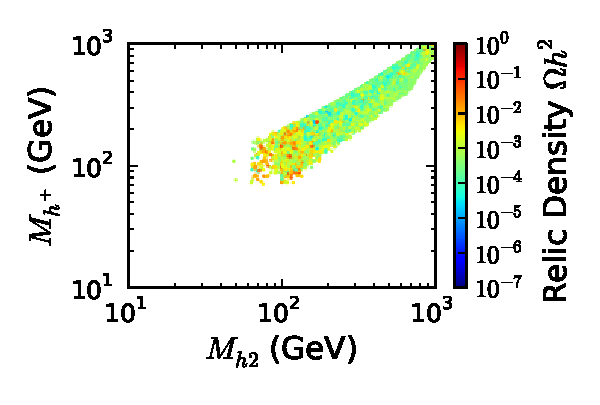
\includegraphics[width=0.41\textwidth]{Figures/Mhc_Mh2_Omega_large-cut1234567.pdf}}%
\vskip -1.05cm
\hspace*{1.2cm}(g)\hspace*{0.35\textwidth}\hspace*{-1.3cm}(h)\hspace*{0.35\textwidth}\hspace*{-1.2cm}(i)
\vskip 0.0cm
{\hspace*{-0.3cm}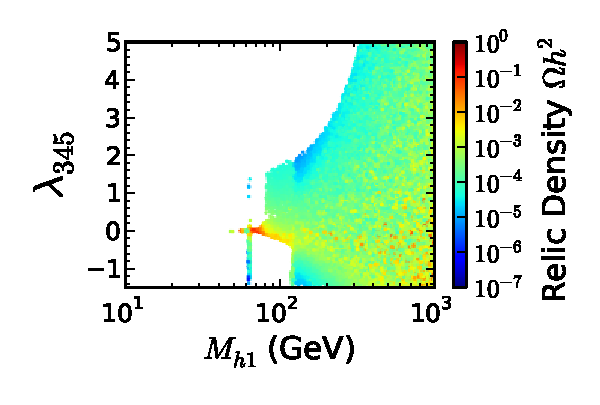
\includegraphics[width=0.41\textwidth]{Figures/Mh1_ld345_Omega_large-cut12345678.pdf}}%
{\hspace*{-1.78cm}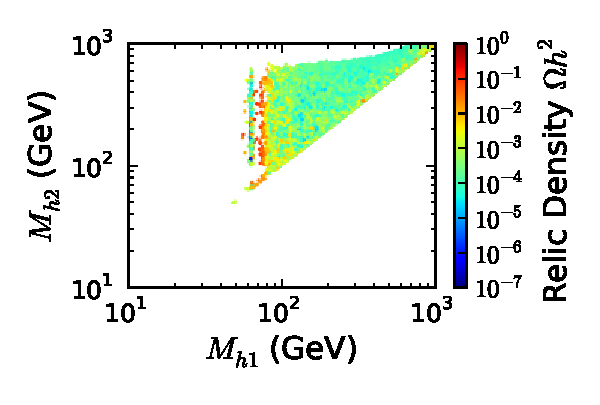
\includegraphics[width=0.41\textwidth]{Figures/Mh1_Mh2_Omega_large-cut12345678.pdf}}%
{\hspace*{-1.77cm}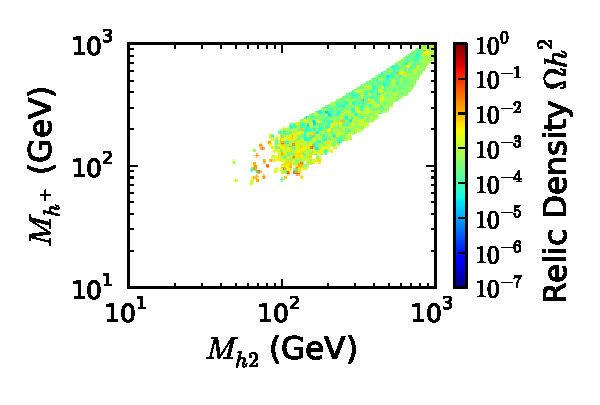
\includegraphics[width=0.41\textwidth]{Figures/Mhc_Mh2_Omega_large-cut12345678.pdf}}%
\vskip -1.05cm
\hspace*{1.2cm}(j)\hspace*{0.35\textwidth}\hspace*{-1.3cm}(k)\hspace*{0.35\textwidth}\hspace*{-1.2cm}(l)
\caption{Colour maps of DM relic density for 2D projections of the 5D random scan of the i2HDM:  
each row demonstrates the effect of consequent application
of the experimental and theoretical constraints in the $(M_{h_1},\lambda_{345})$, $(M_{h_1},M_{h_2})$ and 
$(M_{h_1},M_{h^{+}})$ planes. Each row correspond to the Cut-1-4, described in the text: Cut-1 for (a-c) [Eq.s(\ref{eq:scalar-pot1}-\ref{eq:l345min})]; Cut-2 for (d-f) [Eq.s(\ref{eq:constr-widths}),(\ref{eq:dmh12}),(\ref{eq:ewpt}),(\ref{eq:lhc-higgs-invis}-\ref{eq:lhc-higgs-aa})]; Cut-3 for (g-i) [$\Omega_{\rm DM}^{\rm Planck} h^2 \le 0.1184+2\times 0.0012$]; Cut-4 for (j-l) [LUX].
%
%The first row --  the parameter space after the requirement of vacuum stability 
%[Eq.(\ref{eq:scalar-pot1}-\ref{eq:scalar-pot2},\ref{eq:l345max})], perturbativity  and unitarity
%[Eq.(\ref{eq:pert}-\ref{eq:l345min})]; the second row --   after additional constraints from LEP
%[Eq.~(\ref{eq:constr-widths}),(\ref{eq:dmh12})], EWPT [Eq.~(\ref{eq:ewpt}] and the LHC Higgs data
%[Eq.~(\ref{eq:lhc-higgs-invis}-\ref{eq:lhc-higgs-aa})]; the third row --   after  additional constraint on relic
%density [$\Omega_{\rm DM}^{\rm Planck} h^2 \le 0.1184+2\times 0.0012$]; the fourth row --  after additional
%constraints from DM DD searches from LUX.
\label{fig:dm-i2hdm}} 
\end{figure}
%
%
%
\begin{figure}[htb]
\vskip -1.0cm
\hspace*{-0.3cm}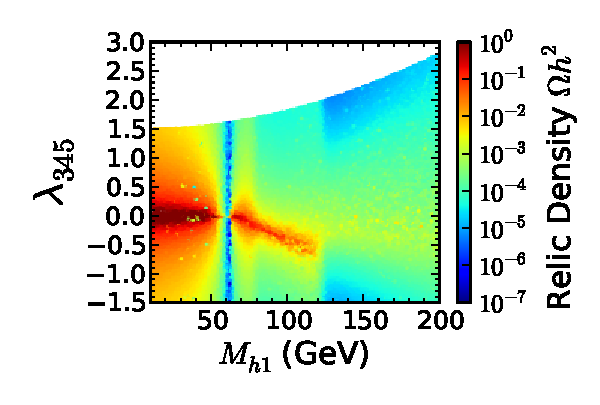
\includegraphics[width=0.4\textwidth]{Figures/Mh1_ld345_Omega_small-cut12_z.pdf}%
\hspace*{-1.55cm}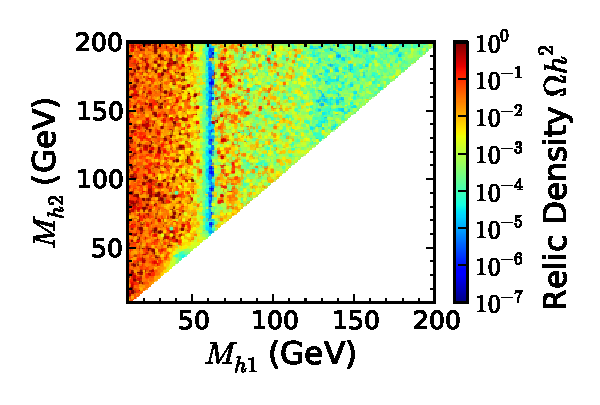
\includegraphics[width=0.4\textwidth]{Figures/Mh1_Mh2_Omega_small-cut12_z.pdf}%
\hspace*{-1.55cm}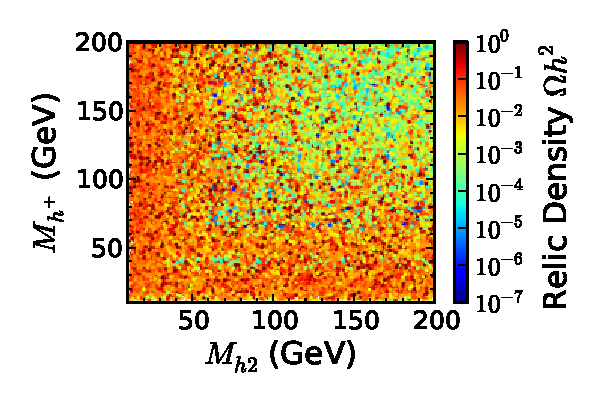
\includegraphics[width=0.4\textwidth]{Figures/Mhc_Mh2_Omega_small-cut12_z.pdf}%
\vskip -5.2cm
\hspace*{4.9cm}
\includegraphics[width=0.55cm,height=4.cm]{Figures/blank.pdf}%
\hspace*{4.9cm}
\includegraphics[width=0.55cm,height=4.cm]{Figures/blank.pdf}%
\vskip 0.2cm
\hspace*{1.4cm}(a)\hspace*{0.35\textwidth}\hspace*{-1.4cm}(b)\hspace*{0.35\textwidth}\hspace*{-1.5cm}(c)
\vskip  0.0cm
%
{\hspace*{-0.3cm}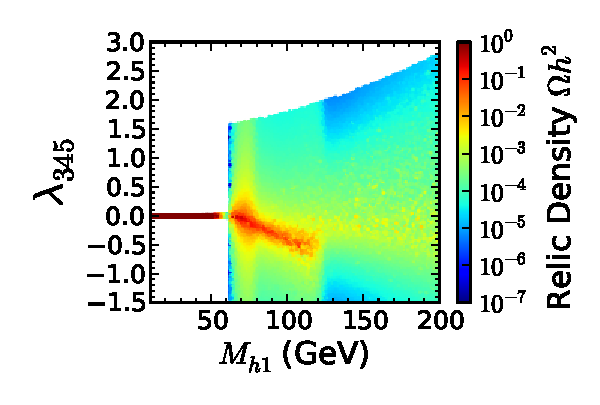
\includegraphics[width=0.4\textwidth]{Figures/Mh1_ld345_Omega_small-cut123456_z.pdf}}%
{\hspace*{-1.55cm}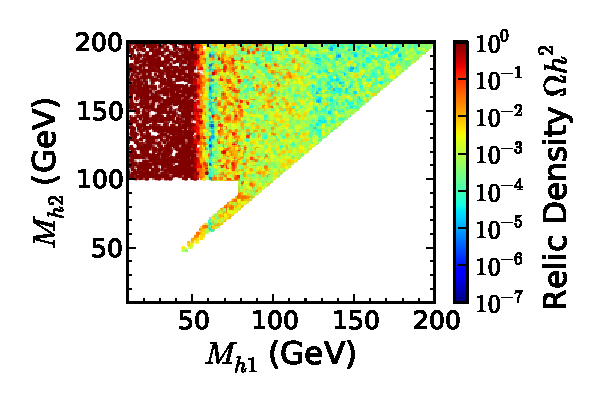
\includegraphics[width=0.4\textwidth]{Figures/Mh1_Mh2_Omega_small-cut123456_z.pdf}}%
{\hspace*{-1.55cm}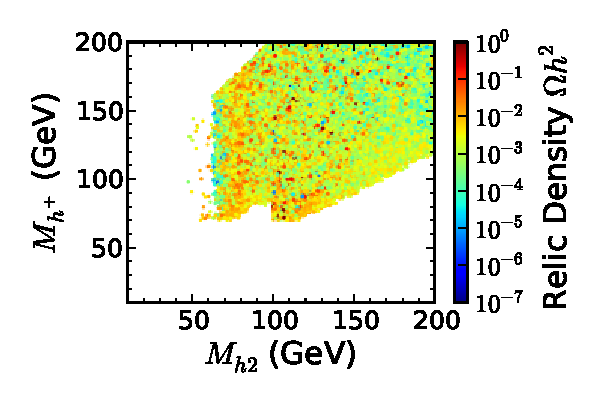
\includegraphics[width=0.4\textwidth]{Figures/Mhc_Mh2_Omega_small-cut123456_z.pdf}}%
\vskip -5.2cm
\hspace*{4.9cm}
\includegraphics[width=0.55cm,height=4.cm]{Figures/blank.pdf}%
\hspace*{4.9cm}
\includegraphics[width=0.55cm,height=4.cm]{Figures/blank.pdf}%
\vskip 0.2cm
\hspace*{1.4cm}(d)\hspace*{0.35\textwidth}\hspace*{-1.4cm}(e)\hspace*{0.35\textwidth}\hspace*{-1.5cm}(f)
\vskip 0.0cm
%
{\hspace*{-0.3cm}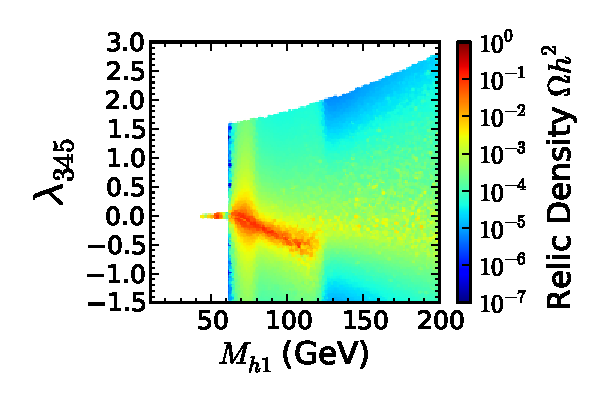
\includegraphics[width=0.4\textwidth]{Figures/Mh1_ld345_Omega_small-cut1234567_z.pdf}}%
{\hspace*{-1.55cm}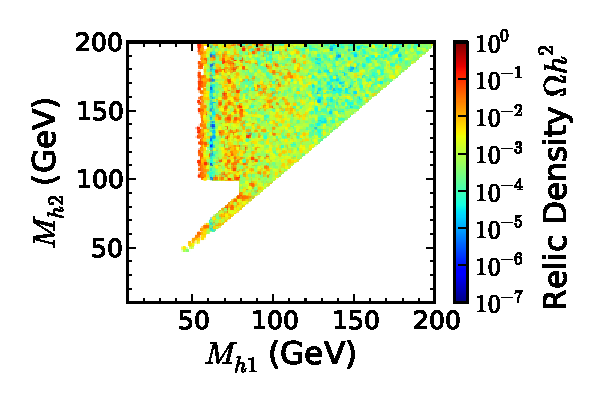
\includegraphics[width=0.4\textwidth]{Figures/Mh1_Mh2_Omega_small-cut1234567_z.pdf}}%
{\hspace*{-1.55cm}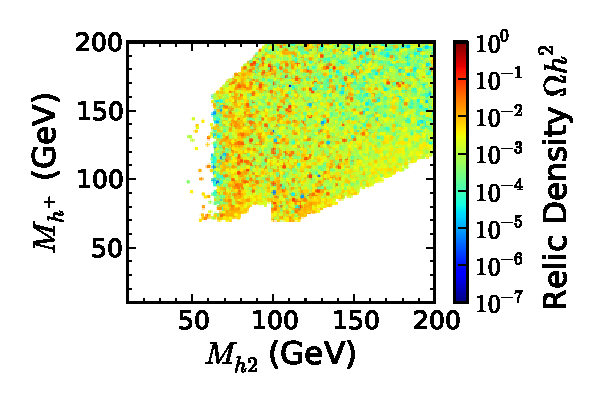
\includegraphics[width=0.4\textwidth]{Figures/Mhc_Mh2_Omega_small-cut1234567_z.pdf}}%
\vskip -5.2cm
\hspace*{4.9cm}
\includegraphics[width=0.55cm,height=4.cm]{Figures/blank.pdf}%
\hspace*{4.9cm}
\includegraphics[width=0.55cm,height=4.cm]{Figures/blank.pdf}%
\vskip 0.2cm
\hspace*{1.4cm}(g)\hspace*{0.35\textwidth}\hspace*{-1.5cm}(h)\hspace*{0.35\textwidth}\hspace*{-1.6cm}(i)
\vskip 0.0cm
{\hspace*{-0.3cm}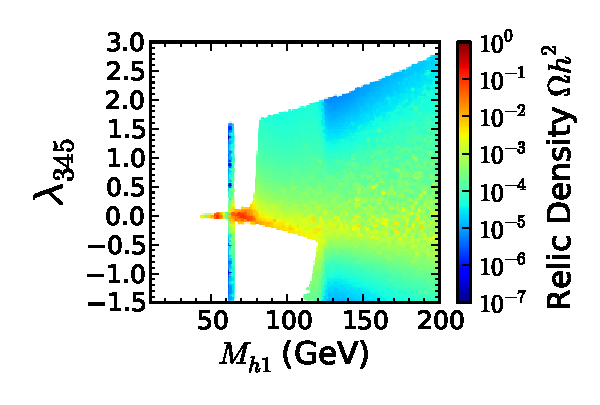
\includegraphics[width=0.4\textwidth]{Figures/Mh1_ld345_Omega_small-cut12345678_z.pdf}}%
{\hspace*{-1.55cm}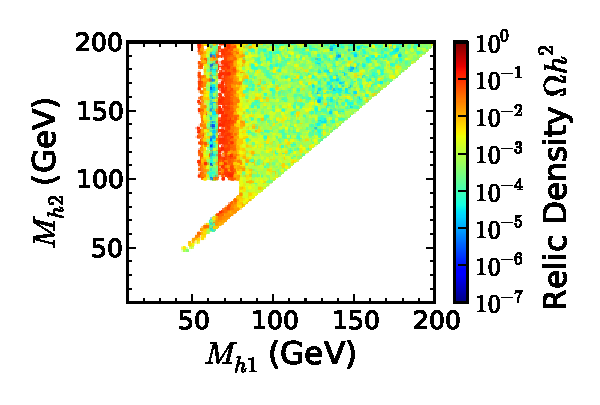
\includegraphics[width=0.4\textwidth]{Figures/Mh1_Mh2_Omega_small-cut12345678_z.pdf}}%
{\hspace*{-1.55cm}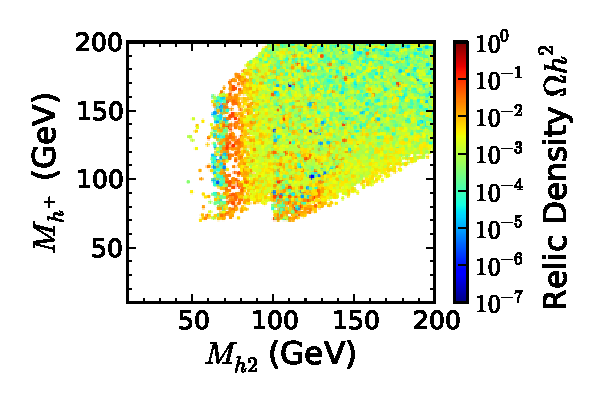
\includegraphics[width=0.4\textwidth]{Figures/Mhc_Mh2_Omega_small-cut12345678_z.pdf}}%
\vskip -5.2cm
\hspace*{4.9cm}
\includegraphics[width=0.55cm,height=4.cm]{Figures/blank.pdf}%
\hspace*{4.9cm}
\includegraphics[width=0.55cm,height=4.cm]{Figures/blank.pdf}%
\vskip 0.2cm
\hspace*{1.4cm}(j)\hspace*{0.35\textwidth}\hspace*{-1.5cm}(k)\hspace*{0.35\textwidth}\hspace*{-1.6cm}(l)
\caption{Colour maps of DM relic density for 2D projections of the 5D random scan of the
i2HDM for the parameter space restricted to (10 GeV - 200 GeV) for $M_{h_1},M_{h_2}$ and
$M_{h^{+}}$. As for Fig.~\ref{fig:dm-i2hdm} each row correspond to the Cut-1-4, described in the text: Cut-1 for (a-c) [Eq.s(\ref{eq:scalar-pot1}-\ref{eq:l345min})]; Cut-2 for (d-f) [Eq.s(\ref{eq:constr-widths}),(\ref{eq:dmh12}),(\ref{eq:ewpt}),(\ref{eq:lhc-higgs-invis}-\ref{eq:lhc-higgs-aa})]; Cut-3 for (g-i) [$\Omega_{\rm DM}^{\rm Planck} h^2 \le 0.1184+2\times 0.0012$]; Cut-4 for (j-l) [LUX].\label{fig:dm-i2hdm-small}}
\end{figure}

The results of the  scan are  presented in Fig.~\ref{fig:dm-i2hdm} in the form of a colour map of
DM relic density, projected on two-dimensional planes: $(M_{h_1},\lambda_{345})$ in the first,
$(M_{h_1},M_{h_2})$ in the second, and $(M_{h_2},M_{h^{+}})$ in the third column, respectively.
The four rows reproduce the effect of the progressive application of the four Cuts defined above.
In Fig.~\ref{fig:dm-i2hdm-small} we also present, in the same format, the results of a finer scan, zoomed to the region of low masses, where the range has been restricted to $10$--$200$ GeV for the three masses $M_{h_1},M_{h_2}$ and $M_{h^{+}}$. The latter is the most relevant corner of parameter space for the LHC phenomenology that we will discuss in the next section. Note that the lower bound of $\lambda_{345}$ presented in these plots corresponds to the lowest limits allowed by unitarity, perturbativity and scalar potential constraints (see Fig.~\ref{fig:par-space1}).

% where  each row demonstrates the effect of step-by-step application of the
%experimental and theoretical constraints, while different columns show  2-d planes  for
%different pairs of the model parameters. The first row -- Figs.\ref{fig:dm-i2hdm} (a-c)
%presents the parameter space after the requirement of vacuum stability 
%[Eq.(\ref{eq:scalar-pot1}-\ref{eq:scalar-pot2},\ref{eq:l345max})], perturbativity  and
%unitarity [Eq.(\ref{eq:pert}-\ref{eq:l345min})] in $(M_{h_1}-\lambda_{345})$,
%$(M_{h_1}-M_{h_2})$ and  $(M_{h_2}-M_{h^{+}})$ planes  respectively. The second row --  
%Figs.\ref{fig:dm-i2hdm}(d-f) -- presents results for the same planes  after additional
%constraints from LEP [Eq.~(\ref{eq:constr-widths}),(\ref{eq:dmh12})], EWPT
%[Eq.~(\ref{eq:ewpt}] and the LHC Higgs data
%[Eq.~(\ref{eq:lhc-higgs-invis}-\ref{eq:lhc-higgs-aa})]. The third row --  
%Figs.\ref{fig:dm-i2hdm}(g-i) -- presents results after  additional constraint on relic
%density  [$\Omega_{\rm DM}^{\rm Planck} h^2 \le 0.1184+2\times 0.0012$] and, finally, the
%fourth row --   Figs.\ref{fig:dm-i2hdm}(j-l) -- presents results after additional constraints
%from DM DD searches from LUX. We will denote the constraints for each row of
%Fig.\ref{fig:dm-i2hdm} by Cut$\#1$-Cut$\#4$ respectively, noting that each  next cut includes
%the previous one.
%At the same time in Figs.\ref{fig:dm-i2hdm-small} we have presented analogous results
%for the 'zoomed' parameter space  restricted to (10 GeV - 200 GeV) for $M_{h_1},M_{h_2}$ and $M_{h^{+}}$
%relevant to collider phenomenology as we discuss below.



One can see from Figs.~\ref{fig:dm-i2hdm}-\ref{fig:dm-i2hdm-small}(a) that $\lambda_{345}$ is limited from above,
and the dependence which defines the  shape of this limit as a function of $M_{h_1}$ comes from 
the vacuum stability condition given by Eq.(\ref{eq:l345max}). One can also see from
Figs.~\ref{fig:dm-i2hdm}-\ref{fig:dm-i2hdm-small}(a), (b), and analogous figures in the rows below, that the relic density
is too high for small $M_{h_1}$ values and small $\lambda_{345}$.
Therefore, the relic density
constraint combined with the LHC Higgs data constraints (limiting the invisible decays of the Higgs) restricts $M_{h_1}$ to be above 45 GeV,
as it can be clearly seen from 
Figs.~\ref{fig:dm-i2hdm}-\ref{fig:dm-i2hdm-small}(g) and (h).
For example, the range 45 GeV $<M_{h_1}<$ 50 GeV is allowed but it requires $h_1h_2$ co-annihilation
and respective mass degeneracy, as one can see from Figs.~\ref{fig:dm-i2hdm}-\ref{fig:dm-i2hdm-small}(h) and (k). From
Figs.~\ref{fig:dm-i2hdm}-\ref{fig:dm-i2hdm-small}(a), (b) and analogous ones in the rows below, one can see a clear vertical blue
pattern of low relic density corresponding to the $h_1 h_1 \to H$ resonant annihilation.  For $M_{h_1}>M_H/2$
the pattern of DM relic density follows the pattern of  $WW$, $ZZ$ and $HH$ thresholds 
presented earlier in Fig.~\ref{fig:1d-mh1-Omega}.

One can also observe that the effect of Cut-1 plus Cut-2 is quite dramatic: a)
$Br(H\to h_1 h_1)<0.28$ and $\mu^{\gamma\gamma} = 1.14^{+0.38}_{-0.36}$ constraints
require $\lambda_{345}\leq 0.02$ for $M_{h_1}<M_H/2$
[Figs.~\ref{fig:dm-i2hdm}-\ref{fig:dm-i2hdm-small}(d)]; b) LEP constraints require $M_{h_2}\gtrsim 100$ GeV if 
$M_{h_2}-M_{h_1}>8$~GeV [Figs.~\ref{fig:dm-i2hdm}-\ref{fig:dm-i2hdm-small}(e)]; c) LEP and LHC Higgs data constraints 
require  $M_{h^+}>70$~GeV, while $M_{h_2}$ is generically excluded below $M_Z/2$ [Figs.~\ref{fig:dm-i2hdm}-\ref{fig:dm-i2hdm-small}(f)].
The effect from adding the (upper) cut from relic density (Cut-3)
is shown in Figs.~\ref{fig:dm-i2hdm}-\ref{fig:dm-i2hdm-small}(g-i): one can see that this cut
(combined with the previous ones)
excludes $M_{h_1}<M_Z/2$
for the whole i2HDM parameter space [Figs.~\ref{fig:dm-i2hdm}-\ref{fig:dm-i2hdm-small}(g,h)],
but does not have a visible effect in  $(M_{h_2},M_{h^{+}})$ plane [Fig.\ref{fig:dm-i2hdm}-\ref{fig:dm-i2hdm-small}(i)].
Actually the  region with $M_{h_1}<M_Z/2$ is excluded due to the interplay of several constraints.
In the  $M_{h_1}<M_H/2$ region with $|\lambda_{345}|\lesssim 0.02$ as required by LHC Higgs data,
the only possibility for relic density of $h_1$ to be sufficiently low to satisfy the PLANCK constraints
is the $h_1 h_2$ co-annihilation channel:
potentially this co-annihilation could provide low enough relic density 
for $M_{h_1}$ down to about 20 GeV. However,  for $M_{h_1}+M_{h_2}< M_Z$
the $Z\to h_1 h_2$ decay is open and contributes significantly to the invisible
Z-boson decay, that is strongly limited by LEP. As the $Z$-boson partial width for this decay channel
is defined just by $M_{h_1}$ and $M_{h_2}$, since $Z h_1 h_2$ coupling is fixed by the gauge invariance,
the $M_{h_1}+M_{h_2}< M_Z$ parameter space is completely excluded. 
For  $h_1 h_2$ co-annihilation region, this exclusion is equivalent to   $M_{h_1}, M_{h_2} \gtrsim M_Z/2$.
The $h_1 h_2$ co-annihilation corridor which provides relic density
below or equal to PLANCK limit is clearly visible in Figs.~\ref{fig:dm-i2hdm}-\ref{fig:dm-i2hdm-small}(e,h,k).

The additional constraint from DM DD from LUX (Cut-4)
removes a substantial portion of the  parameter space for large and intermediate $|\lambda_{345}|$
values for $M_{h_1}\lesssim M_H$  [Figs.~\ref{fig:dm-i2hdm}-\ref{fig:dm-i2hdm-small}(j)].
In this excluded parameter space the scattering cross section of $h_1$ on the proton 
is quite large due to the Higgs boson exchange enhanced by $|\lambda_{345}|$, while the relic density is respectively low,
again due to the large value  $|\lambda_{345}|$, but it is not low enough to suppress
the DM detection rate below the experimental exclusion.
So, the LUX cut removes the low relic density region, 
and one can see this clearly in Figs.~\ref{fig:dm-i2hdm}-\ref{fig:dm-i2hdm-small}(k-l)
by the enhanced yellow-red colour in the $M_{h_1}\lesssim M_H$ region 
in comparison to the respective Figs.~\ref{fig:dm-i2hdm}-\ref{fig:dm-i2hdm-small}(h-i)
where the DM DD cut was not applied.
For $\lambda_{345} \gtrsim 0.2$ the parameter space is excluded
for $M_H/2<M_{h_1}<M_W$ while for  $\lambda_{345} \lesssim -0.2$
it is excluded for $M_H/2<M_{h_1}<M_H$ as illustrated in Figs.~\ref{fig:dm-i2hdm}-\ref{fig:dm-i2hdm-small}(j).
Once the $h_1 h_1 \to W^+ W^-$ channel is open for positive  $\lambda_{345}$,
or $h_1 h_1 \to H H$ channel is open for negative $\lambda_{345}$,
the relic density drops substantially below the PLANCK limit, which makes the rescaling factor 
low enough to avoid limits from LUX searches.
The difference between the positive and negative $\lambda_{345}$ cases
is related to the respective positive and negative interference of
$h_1 h_1 \to H \to X X$ channel with non-Higgs-exchange diagrams.
This asymmetry between positive and negative $\lambda_{345}$ cases was seen initially
in Fig.~\ref{fig:1d-mh1-Omega}, where the $h_1$ relic density was presented as a function 
of $M_{h_1}$ for different $\lambda_{345}$ values.

In summary, after all constraints given by Cut-1-Cut-4,
we found that the parameter space with  
\begin{equation}
M_{h_1},M_{h_2}<45~\mbox{GeV} 
\mbox{\ or\ } M_{h^+}<70~\mbox{GeV} 
\label{eq:exclusion1}
\end{equation}
is completely excluded. Our results  agree with the results of previous studies on the i2HDM (see, e.g., \cite{Arhrib:2013ela,Ilnicka:2015jba}).
In particular, authors of \cite{Ilnicka:2015jba} have also stated 
the $M_{h_1},M_{h_2}<45~\mbox{GeV}$ limit.
However we would like to stress that the general exclusion 
for $M_{h_1},M_{h_2}$ {\it and for} $M_{h^+}$
given by Eq.~(\ref{eq:exclusion1}) is established here for the first time, to the best of our knowledge. In~\cite{Ilnicka:2015jba}, for example,  the authors demonstrate 
(see Fig.~6 and Eq.~(18) in \cite{Ilnicka:2015jba}) that 
$M_{h^+}$ above $M_H$ is excluded from a  specific scan. Here we find that
$M_{h^+}$ as light as 70 GeV  is allowed by all present constraints, while $M_{h_1}$ and
$M_{h_2}$ are generically allowed to be as light as 45 GeV. One should note that specific regions of the
parameter space can be excluded using di-lepton and missing transverse momentum
signatures: for example, in a recent study~\cite{Belanger:2015kga} the authors showed that values of the masses below
$M_{h_1}\lesssim 50$~GeV and  $M_{h_2}\lesssim 140$~GeV can be excluded using this signature,
provided that the mass gap between $M_{h_2}$ and $M_{h_1}$ is large enough. However, we find that this parameter
space region is already excluded by the upper cut on the relic density (Cut-3), as one can see
from Fig.~\ref{fig:dm-i2hdm-small}(h): for  $M_{h_2}>100$~GeV, the entire region $M_{h_1}\lesssim
50$~GeV  is excluded by Cut-3 combined with previous cuts (including LEPII limits).

We would also like to point to some features of the scan for  the region of $M_{h_1},M_{h_2}$ and
$M_{h^{+}}$ above 200 GeV, presented  in Fig.~\ref{fig:dm-i2hdm}. From 
Figs.~\ref{fig:dm-i2hdm}(f),(i),(l), one can see that EWPT constraints require a very  modest
mass split between $M_{h_2}$ and $M_{h^{+}}$ since this mass split is directly related to
values of the $M_{h_2}$ and $M_{h^{+}}$ couplings to  the SM Higgs as well as to the couplings
to longitudinal components of the W and Z-bosons. Therefore constraints from $S$ and $T$
parameters leave only a rather narrow corridor in the  ($M_{h^{+}},M_{h_2}$) plane.


%%%%%%%%%%%%%%%%%%%%%%%%%%%
\subsection{Fitting the relic density}


In our analysis, we generically allow the DM relic density to be equal or
below the PLANCK constraints, Eq.~(\ref{eq:planck-limit}).
This is the concept of our approach: we assume that in the case of under-abundance
there should be either additional sources of DM or mechanisms other than thermal freeze-out that 
compensate for the DM deficit, such as DM freeze-in scenarios~\cite{Hall:2009bx}.
Keeping this in mind, we exclude in our analysis only those regions of the parameter space 
where the relic density exceeds the PLANCK constraint.
It is however instructive to explore also the parameter space where both
the upper and lower PLANCK limits are satisfied.
This parameter space region is presented for the ``full'' scan 10 GeV $< M_{h_1}, M_{h_2}, M_{h^{+}} < 1000$~GeV
in Fig.~\ref{fig:dm-i2hdm-relic} and for the ``zoomed'' scan 10 GeV $< M_{h_1}, M_{h_2}, M_{h^{+}} < 200$~GeV in Fig.~\ref{fig:dm-i2hdm-relic-small}.

\begin{figure}[htb]
\hspace*{-0.2cm}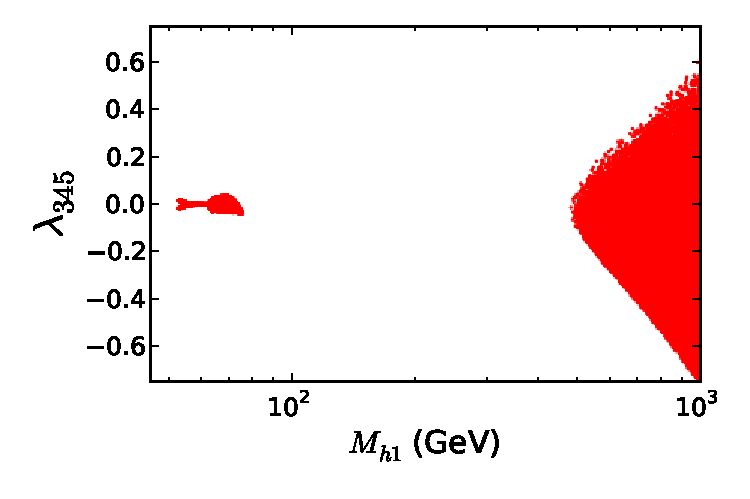
\includegraphics[width=0.50\textwidth]{Figures/Mh1_ld345_Omega_zoom-cut123456789_zz-large-monoc.pdf}%
\hspace*{-0.2cm}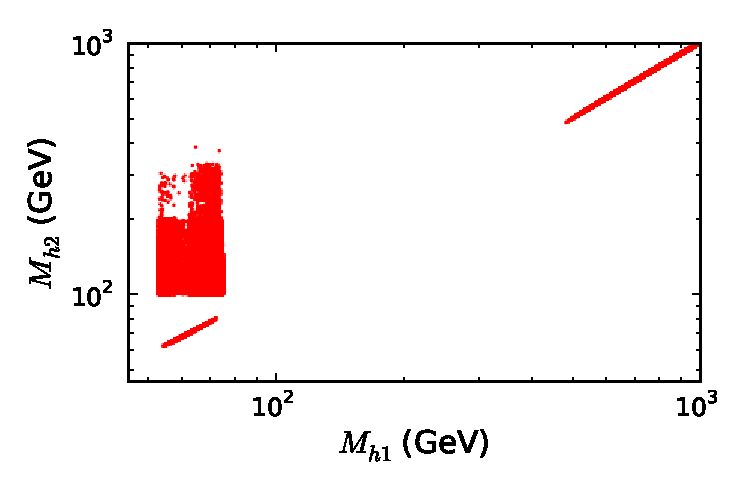
\includegraphics[width=0.50\textwidth]{Figures/Mh1_Mh2_Omega_zoom-cut123456789_zz-large-monoc.pdf}
\vskip -1.0cm
\hspace*{1cm}(a)\hspace*{0.55\textwidth}\hspace*{-1.5cm}(b)
\\
\\
\hspace*{-0.2cm}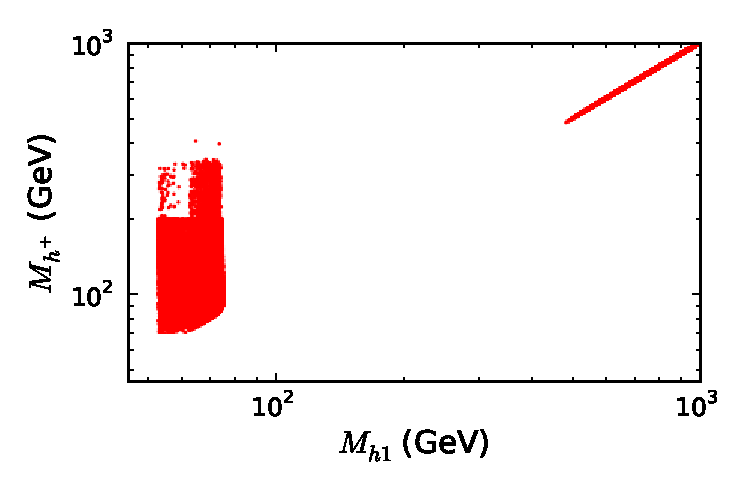
\includegraphics[width=0.50\textwidth]{Figures/Mh1_Mhc_Omega_zoom-cut123456789_zz-large-monoc.pdf}%
\hspace*{-0.2cm}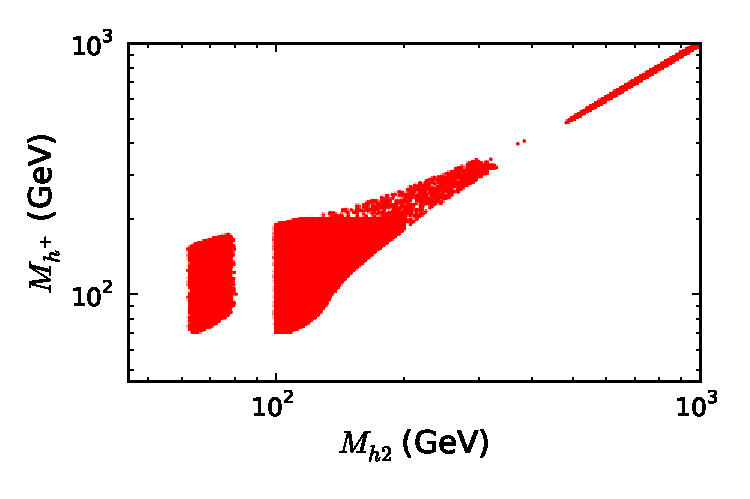
\includegraphics[width=0.50\textwidth]{Figures/Mhc_Mh2_Omega_zoom-cut123456789_zz-large-monoc.pdf}
\vskip -1.0cm
\hspace*{1cm}(c)\hspace*{0.55\textwidth}\hspace*{-1.5cm}(d)
\caption{2D projections of the 5D random scan of the i2HDM for
 the ``full'' parameter space 10 GeV $< M_{h_1}, M_{h_2}, M_{h^{+}} < 1000$~GeV
satisfying all constraints (Cut-1 to Cut-4) considered above for Fig.~\ref{fig:dm-i2hdm},\ref{fig:dm-i2hdm-small}
plus a lower constraint on relic density given by  Eq.(\ref{eq:planck-limit})}
\label{fig:dm-i2hdm-relic}
\end{figure}
%
\begin{figure}[htb]
\hspace*{-0.2cm}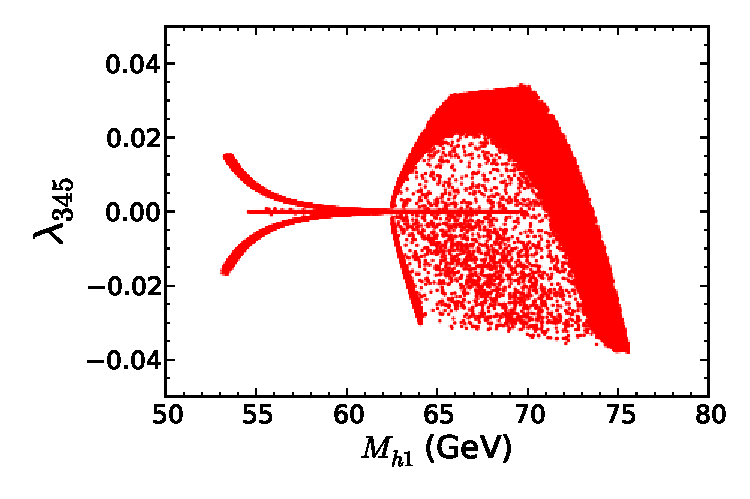
\includegraphics[width=0.50\textwidth]{Figures/Mh1_ld345_Omega_zoom-cut123456789_zz-monoc.pdf}%
\hspace*{-0.2cm}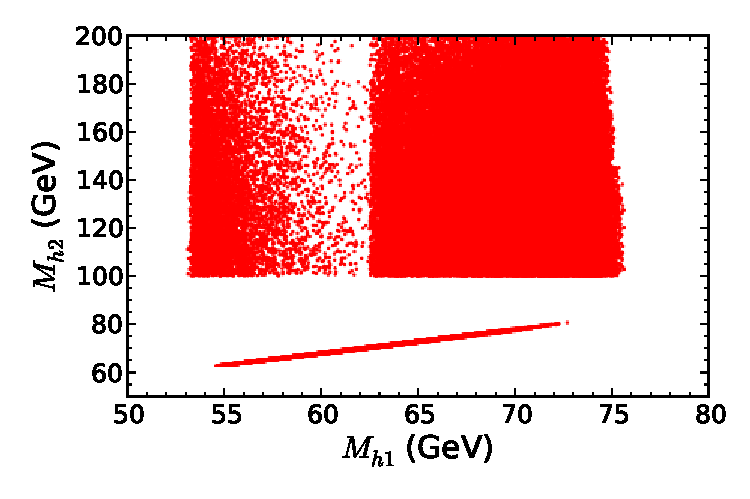
\includegraphics[width=0.50\textwidth]{Figures/Mh1_Mh2_Omega_zoom-cut123456789_zz-monoc.pdf}
\vskip -0.8cm
\hspace*{1cm}(a)\hspace*{0.55\textwidth}\hspace*{-1.5cm}(b)
\\
\\
\hspace*{-0.2cm}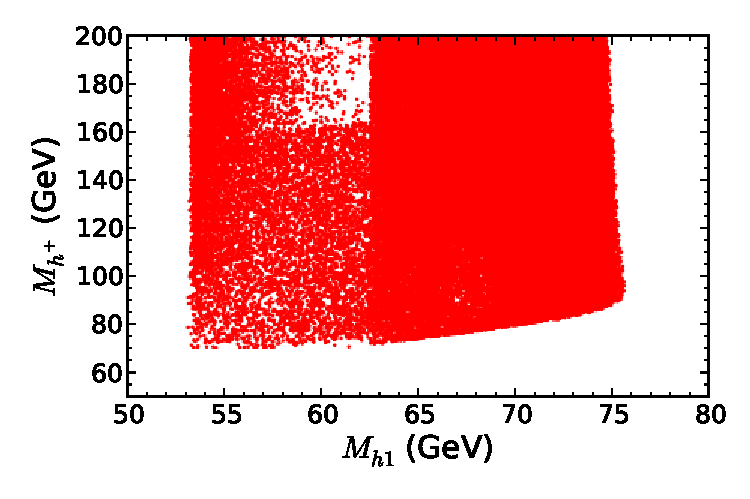
\includegraphics[width=0.50\textwidth]{Figures/Mh1_Mhc_Omega_zoom-cut123456789_zz-monoc.pdf}%
\hspace*{-0.2cm}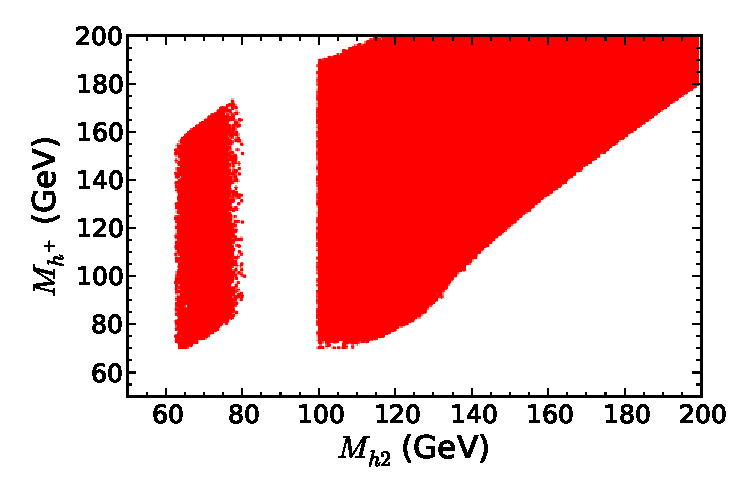
\includegraphics[width=0.50\textwidth]{Figures/Mhc_Mh2_Omega_zoom-cut123456789_zz-monoc.pdf}
\vskip -0.8cm
\hspace*{1cm}(c)\hspace*{0.55\textwidth}\hspace*{-1.5cm}(d)
\caption{2D projections of the 5D random scan of the i2HDM for the ``zoomed'' parameter space
10 GeV $< M_{h_1}, M_{h_2}, M_{h^{+}} < 200$~GeV satisfying all constraints
(Cut-1 to Cut-4) considered above for Fig.~\ref{fig:dm-i2hdm},\ref{fig:dm-i2hdm-small} plus a
lower constraint on relic density given by  Eq.(\ref{eq:planck-limit})}
\label{fig:dm-i2hdm-relic-small}
\end{figure}

Many interesting features of the i2HDM parameter space arise from Figs.~\ref{fig:dm-i2hdm-relic} and~\ref{fig:dm-i2hdm-relic-small} once the
``correct'' amount of DM relic density is required. 
The $(\lambda_{345},M_{h_1})$ plane shown in Fig.~\ref{fig:dm-i2hdm-relic}(a) displays only two very distinctive $M_{h_1}$ regions 
where the relic density satisfies the PLANCK limit within 2 standard deviations. 
The first region at low masses, $53~\mbox{GeV} \lesssim
M_{h_1} \lesssim 76~\mbox{GeV}$, is presented in finer detail in
Fig.~\ref{fig:dm-i2hdm-relic-small}. 
%The second one is realised for $M_{h_1}\gtrsim 490\mbox{GeV}$. 
%The first region presented in details in Fig.~\ref{fig:dm-i2hdm-relic-small} consists of several parts:
It clearly shows the presence of various regions with specific physical properties:
\begin{itemize}
\item[a)] For $M_{h_1}< M_H/2$, three thin strips are observed. The two symmetric wings for positive and negative $\lambda_{345}$ 
clearly visible in Fig.~\ref{fig:dm-i2hdm-relic-small}(a) correspond to DM annihilation via the Higgs boson exchange. 
The thin horizontal line for very small values of $\lambda_{345}$ corresponds to the $h_1h_2$ co-annihilation. 
The latter can also be seen in Fig.~\ref{fig:dm-i2hdm-relic-small}(b) as a thin diagonal strip at low $M_{h_2}$
starting from 54 GeV and extending beyond $M_H/2$ up to about 73 GeV.
%
%
%is split in two two parts in its turn -- the one 
%which  presents  DM annihilation channel trough the Higgs boson exchange
%and has a shape of two symmetric wings for negative and positive values of $\lambda_{345}$
%(Fig.~\ref{fig:dm-i2hdm-relic-small}(a))
%and the other which presented by the thin horizontal strip in
%($\lambda_{345} - M_{h_1}$) plane (Fig.~\ref{fig:dm-i2hdm-relic-small}(a))
%as well as  thin  strip in the lower part of (Fig.~\ref{fig:dm-i2hdm-relic-small}(b))
%corresponding to $h_1 - h_2$ annihilation region. This co-annihilation strip
%starts at  54 GeV and goes actually beyond  $M_H/2$ up to 73 GeV.
The width of this strip is defined by 
the maximum allowed value of $\Delta M = M_{h_2}-M_{h_1}=8$~GeV, above which
the parameter space is excluded by LEP di-lepton searches until $M_{h_2} > 100$ GeV (see Eq.~\ref{eq:dmh12}). For  $\Delta M<8$~GeV
and $M_{h_1}<54$~GeV on the other hand, the $\Omega h^2$ is below the PLANCK limit in this region. The upper edge
at $73$ GeV is defined by the rapid increase of the  $h_1 h_1 \to W W^*$ contribution,
which does not require co-annihilation above this mass. The typical $M_{h_2}-M_{h_1}$
mass split in the co-annihilation region is 6-8 GeV, required to make the relic density 
consistent with the Plank limit.
This small, but important region of the parameter space, which is realised for  $\lambda_{345} \simeq 0$
and consistent with all present constraints has been missed in the previous studies.

\item[b)] In the region $M_H/2<  M_{h_1} \lesssim 76~\mbox{GeV}$,  
large absolute values of  $\lambda_{345}$ are allowed by the LHC Higgs data, however LUX data requires $|\lambda_{345}|$ to be below about 0.04.
In this region, we remark the asymmetric pattern in the ($\lambda_{345},M_{h_1}$) plane
for positive and negative values of $\lambda_{345}$, which is related, respectively, to the 
positive and negative interference of  $h_1 h_1 \to VV$ annihilation diagrams ($V=Z,W$) via Higgs boson exchange
and diagrams with quartic $h_1 h_1 V V$  interactions. 
\end{itemize}

\subsection{The high mass region and the LHC sensitivity}

The relic density can also be ``just right'' at large masses $M_{h_1}\gtrsim 490\mbox{ GeV}$, as shown in Fig.~\ref{fig:dm-i2hdm-relic}. 
This high-mass region deserves a separate discussion. 
Its most salient feature is the high degree of degeneracy among the three inert Higgs boson masses, 
as one can see from Fig.~\ref{fig:dm-i2hdm-relic}(b),(c),(d). Numerically we find that the
maximal mass difference among $h_1$, $h_2$ and $h^+$, that we call $\Delta M^{max}$, does not exceed a few GeV. 

Remarkably, the mass split is required to be {\it large enough}, so that the relic density can reach the {\it lower value} of the PLANCK limit: the increase of  the mass
split is, in fact, correlated with the increase of the quartic coupling $h_1 h_1 V_L V_L$ of the DM to longitudinal $Z$ and $W$ bosons,
which enhances the $h_1 h_1$ annihilation cross section, thus bringing
the DM relic density down to within the experimental limits. Due to the connection between the mass split and the $h_1 h_1 V_L V_L$ couplings, 
see Eq.~(\ref{tildelam345}),
this effect is actually stronger than the effect of the
$h_1$, $h_2$ and $h^+$ co-annihilation, which becomes sub-dominant in this high-mass region.
One should also mention that  $\Delta M^{max}$ of the order of few GeV  is {\it generically} not 
small enough to lead to long-lived $h_2$ or $h^+$ at detector level.
However, in the small mass tip, in the interval
$550\mbox{ GeV} \gtrsim M_{h_1}\gtrsim 490\mbox{ GeV}$,  $\Delta M^{max}$ can take values 
about 0.2-0.25~GeV. This specific range of the mass split simultaneously provides an $\Omega_{\rm DM} h^2$ consistent with 
PLANCK constraint and a life-time for $h^+$ large enough to travel about 10 cm or more in the  detector, thus
providing disappearing charged track signatures which have been recently explored  by  CMS~\cite{CMS:2014gxa}
collaboration.

In the limit of $\Delta M/M\ll 1$ the width of  $h^+$ is proportional to  $\Delta M^5/M_W^4$
and for particular values of $\Delta M\simeq 0.2-0.25$~GeV the  life time of  $h^+$ is between 3 and 1 ns.
After evaluation of the  $h^+$ production cross section for  490--550 GeV mass range
and applying efficiency for the  disappearing charged track signatures provided by  CMS~\cite{CMS:2014gxa}
as a function of charged track transverse momentum as well as efficiency for distance travelled by the charge particle,
we have estimated  that CMS@8TeV with 19.5fb$^{-1}$ data excludes  $h^+$  in the 490-550 GeV mass range for   $\Delta M=0.2-0.25$~GeV.
For example, for $m_{h^+}=500$~GeV the sum of the cross section of $pp\to{h^+}{h^-}$ and  $pp\to{h^\pm}{h_{1,2}}$
is about 0.4 fb, and the product of this cross section, the luminosity, and the above efficiencies gives about 2.5 events
which are above 2 event exclusion level.


One should also note that with increasing DM mass, the required split between $h_1$, $h_2$ and $h^+$
increases.
At about 20 TeV for $M_{h_1}$, the DM relic density constraint together with 
requirement of unitarity and perturbativity which are saturated by  $\Delta M^{max}\simeq 10$~GeV,
close the i2HDM parameter space.

%We would like to stress again that we exclude i2HDM parameter space 
%where relic density {\it exceed}  Planck constraint, so parameter space found 
%in both cases  of Figs.~\ref{fig:dm-i2hdm},\ref{fig:dm-i2hdm-small}(a)(j-l) and in
%Figs.\ref{fig:dm-i2hdm-relic},\ref{fig:dm-i2hdm-relic-small}
%is carried on for further analysis.
%In the next section we study  implications of dedicated DM searches at the LHC 
%which further restrict i2HDM parameter space.
